

\documentclass[11pt]{article}
\documentclass[11pt]{article}
\usepackage[margin=1in]{geometry}
\usepackage{amsmath,amssymb,amsthm,mathtools}
\usepackage{stmaryrd}
\usepackage{mathrsfs}
\usepackage{thmtools}
\usepackage{enumitem}
\usepackage{microtype}
\usepackage[hidelinks]{hyperref}
\usepackage{cleveref}
\usepackage{tikz}
\usetikzlibrary{arrows.meta,positioning,calc}
\usepackage{tikz-cd}
\usepackage{algorithm}
\usepackage[noend]{algpseudocode}
\usepackage{booktabs}

\title{\textbf{Transform--Control UX (TCX):}\\
\Large A Typed, Contract--Indexed, Graded--Effect Calculus for\\ Safe--by--Construction Human--Agent Interaction}
\author{Assistant (first), Jacob Elliott (second)}
\date{Version v0.1 (steelmanned) --- \today}

% Theorem environments
\theoremstyle{definition}
\newtheorem{definition}{Definition}[section]
\newtheorem{example}[definition]{Example}
\theoremstyle{plain}
\newtheorem{theorem}[definition]{Theorem}
\newtheorem{lemma}[definition]{Lemma}
\newtheorem{proposition}[definition]{Proposition}
\newtheorem{corollary}[definition]{Corollary}
\theoremstyle{remark}
\newtheorem{remark}[definition]{Remark}

% Macros
\newcommand{\X}{X}
\newcommand{\XX}{\mathcal{X}} % components of state
\newcommand{\V}{\mathcal{V}}
\newcommand{\A}{\mathcal{A}}
\newcommand{\U}{U}
\newcommand{\F}{\mathcal{F}}
\newcommand{\G}{\mathcal{G}}
\newcommand{\B}{\mathcal{B}}
\newcommand{\D}{\mathsf{D}} % distribution monad
\newcommand{\K}{\mathsf{K}} % kernel
\newcommand{\1}{\mathbf{1}}
\newcommand{\iden}{\mathrm{id}}
\newcommand{\supp}{\mathrm{supp}}
\newcommand{\Pow}{\mathcal{P}}
\newcommand{\EE}{\mathbb{E}}
\newcommand{\RR}{\mathbb{R}}
\newcommand{\NN}{\mathbb{N}}
\newcommand{\indicator}[1]{\llbracket #1 \rrbracket}
\newcommand{\pushfwd}{\mathbin{\!\!\;\raisebox{0.2ex}{\small$\ast$}\!}}
\newcommand{\lift}{\mathsf{lift}}
\newcommand{\clamp}{C}
\newcommand{\grade}{\mathsf{r}}

\begin{document}
\maketitle

\begin{abstract}
We present a unified formalism for designing user--visible operations (UI actions, agent steps, macros, automations) as elements of a typed algebra equipped with explicit \emph{contracts}. The core idea is simple: if every primitive operation is certified to preserve a measurable \emph{safe region} $S$ of the global state space, then closure of the algebra under composition and convex choice yields \emph{safe--by--construction} interactions. Partial or underspecified transforms are totalized by \emph{clamps}---deterministic retractions into $S$---so safety is enforced before execution.

We steelman the concept along four axes: (i) a measure--theoretic semantics using Markov kernels over standard Borel spaces; (ii) a categorical view (Kleisli of the distribution monad, safe reflectors) clarifying why closure properties hold; (iii) a type--and--\emph{graded--effect} system that statically enforces invariants and tracks a probabilistic \emph{hazard budget}; and (iv) a practical finite--state compilation validating invariance as forward--closure of a row--stochastic operator. We prove soundness of the static system (\emph{well--typed programs do not leave $S$}), show how observable--layer contracts lift back to concrete states, and derive a tight failure envelope for soft contracts: $\Pr[\text{failure by }T] \le 1-\prod_{t=1}^T (1-\varepsilon_t) \le \sum_t \varepsilon_t$. We also formalize automatic clamp insertion and sketch minimal--clamp synthesis as a constrained optimization (NP--hard in general) with efficient greedy baselines.
\end{abstract}

\section{Introduction and Contributions}
Modern agentic systems and UI macro layers increasingly assemble complex behavior by composing reusable steps (tool calls, policy gates, post--processors). Safety is typically enforced post hoc via runtime heuristics. We propose \emph{Transform--Control UX (TCX)}: design actions as typed transforms with contracts, then \emph{compile} interactions so they are safe--by--construction.

\paragraph{Setting.} Let $(\X,\F)$ be a measurable state space aggregating world state $\Omega$, surfaces $\V$, artifacts $\A$, and session metadata $\U$: $\X \cong \Omega \times \V \times \A \times \U$. A \emph{contract} is a measurable set $S\in\F$ of acceptable states (e.g.\ ``no PII'', toxicity$\le\theta$, audit log grows'').

\paragraph{Transforms.} We model primitives and macros as \emph{Markov kernels} $K:\X\rightsquigarrow \X$ (i.e.\ measurable $x\mapsto K(x)$, where $K(x)$ is a probability measure on $(\X,\F)$). Deterministic steps are kernels $x\mapsto\delta_{\tau(x)}$. Mixtures implement policy--dependent branching.

\paragraph{Contributions.} We consolidate the intuition into a rigorous, deployable calculus:
\begin{enumerate}[leftmargin=*]
  \item \textbf{Semantics:} TCX lives in the Kleisli category of the distribution monad (a Markov category). Composition and convex choice are closed, clamps realize a reflector into the safe subcategory.
  \item \textbf{Static system:} A type--and--graded--effect system $\Gamma\vdash K: S\Rightarrow S\;\triangleright \grade$ ensures invariance of $S$ and tracks soft hazard budgets additively in log--space. We prove preservation (invariance) and progress (totality via clamps).
  \item \textbf{Observable lifting:} When contracts are defined over an observable layer $O:\X\to Y$, safety proofs performed in $Y$ \emph{pull back} to $\X$ via pushforward of kernels.
  \item \textbf{Algorithmics:} We formalize compile--time clamp insertion and show minimal clamp placement is NP--hard; we provide a greedy heuristic and a finite--state checker (row--stochastic matrices) validating forward closure.
\end{enumerate}

\paragraph{Pragmatics.} In the finite--state setting, safety reduces to checking that no probability mass leaks from rows indexed by $S$ into columns indexed by $S^c$. This yields a fast, auditable static build gate. The same algebra extends to continuous spaces when observables are calibrated.

\section{Semantic Foundation}
\subsection{States, Kernels, and Mixtures}
Let $(\X,\F)$ be a standard Borel space. A \emph{Markov kernel} $K:\X\rightsquigarrow \X$ assigns to each $x\in\X$ a probability measure $K(x)$ on $(\X,\F)$ such that for all $A\in\F$, the map $x\mapsto K(x)(A)$ is measurable. Deterministic transforms $\tau:\X\to \X$ embed as $K_\tau(x)=\delta_{\tau(x)}$.

\begin{definition}[Composition, mixture, identity]\label{def:ops}
Given kernels $K_1,K_2:\X\rightsquigarrow\X$, their Kleisli composition $K_2\circ K_1$ is $(K_2\circ K_1)(x)(A):=\int_{\X} K_2(y)(A)\,K_1(x)(dy)$. The identity is $x\mapsto \delta_x$. For measurable weights $\lambda_i:\X\to[0,1]$ with $\sum_i \lambda_i(x)=1$, the \emph{mixture} $\bigoplus_i \lambda_i K_i$ is the kernel $x\mapsto \sum_i \lambda_i(x) K_i(x)$.
\end{definition}

\subsection{Contracts and $\sigma$--Safety}
\begin{definition}[Contract and $\sigma$--safety]\label{def:sigma}
A \emph{contract} is a measurable $S\in\F$. A kernel $K$ is \emph{$\sigma$--safe on $S$} iff for all $x\in S$, $K(x)(S)=1$ (i.e.\ the image measure is supported in $S$). For a deterministic $\tau$, this reduces to $\tau(S)\subseteq S$.
\end{definition}

\begin{theorem}[Closure under composition]\label{thm:closure-comp}
If $K_1,K_2$ are $\sigma$--safe on $S$, then $K_2\circ K_1$ is $\sigma$--safe on $S$.
\end{theorem}
\begin{proof}
For $x\in S$, $K_1(x)$ is supported in $S$; for $y\in S$, $K_2(y)$ is supported in $S$. Thus $(K_2\circ K_1)(x)$ places all mass in $S$.
\end{proof}

\begin{theorem}[Closure under mixture]\label{thm:closure-mix}
If each $K_i$ is $\sigma$--safe on $S$ and $\sum_i\lambda_i(x)=1$, then $\bigoplus_i \lambda_i K_i$ is $\sigma$--safe on $S$.
\end{theorem}
\begin{proof}
For $x\in S$, $K_i(x)(S)=1$; hence $\left(\sum_i \lambda_i(x)K_i(x)\right)(S)=\sum_i\lambda_i(x) = 1$.
\end{proof}

\subsection{Clamps and Totalization}
Partial or underspecified steps arise naturally. We enforce totality and safety via \emph{clamps}.

\begin{definition}[Clamp]\label{def:clamp}
Fix a contract $S\in\F$ and a designated $s_0\in S$. Define $\clamp_S:\X\to S$ by $\clamp_S(x)=x$ if $x\in S$ and $\clamp_S(x)=s_0$ otherwise (measurable on standard Borel $\X$). Its kernel is $K_{\clamp_S}(x)=\delta_{\clamp_S(x)}$.
\end{definition}

More sophisticated clamps project onto $S$ in a metric sense when $S$ is closed in a Polish space; the simple retraction suffices for soundness.

\begin{proposition}[Clamped totalization]\label{prop:totalize}
For any kernel $K:\X\rightsquigarrow \X$, the clamped kernel $K^S := K_{\clamp_S}\circ K$ is total and $\sigma$--safe on $S$.
\end{proposition}
\begin{proof}
By construction, $K_{\clamp_S}(x)$ is supported in $S$ for all $x$. For $x\in S$, $(K_{\clamp_S}\circ K)(x)$ is also supported in $S$.
\end{proof}

\subsection{Observable Layer and Lifting}
Contracts are often stated over an observable $O:\X\to (Y,\G)$ (surface text, classifiers, etc.).

\begin{definition}[Pushforward]\label{def:pushforward}
Given $O:\X\to Y$ measurable and kernel $K$, the pushforward kernel $O\pushfwd K:\X\rightsquigarrow Y$ is $(O\pushfwd K)(x):=K(x)\circ O^{-1}$.
\end{definition}

\begin{proposition}[Lift from observables]\label{prop:lift}
Let $Q\in\G$ and $S:=O^{-1}(Q)$. If for all $x\in S$ we have $(O\pushfwd K)(x)(Q)=1$, then $K$ is $\sigma$--safe on $S$.
\end{proposition}
\begin{proof}
For $x\in S$, $(O\pushfwd K)(x)(Q)=K(x)(O^{-1}(Q))=K(x)(S)=1$.
\end{proof}

\section{A Typed, Graded--Effect System}
We formalize static checking as a refinement type system that enforces invariance $\{S\}\ K\ \{S\}$ and tracks a soft hazard budget.

\subsection{Judgments and Grades}
We write $\Gamma\vdash K:S\Rightarrow S\;\triangleright \grade$ meaning: under environment $\Gamma$, $K$ preserves $S$ and consumes hazard grade $\grade\in[0,\infty)$ (log--space). Grades compose additively; the probability bound is $1-e^{-\grade}$. Intuitively, if a step has per--apply hazard $\varepsilon$ (leak probability into $S^c$), we set $\grade=-\log(1-\varepsilon)$.

\begin{definition}[Effect algebra]\label{def:effect}
Let $(\RR_{\ge 0},+,0,\le)$ index effects. Define $\phi(\grade)=1-e^{-\grade}$ as the probability bound map. Composition uses addition, mixture uses convexity, and subeffecting is monotone in $\grade$.
\end{definition}

\subsection{Typing Rules}
Let $\lambda_i$ be measurable with $\sum_i\lambda_i(x)=1$. We adopt the following rules:
\begin{align*}
\textbf{[ID]}&\ \ \ \frac{}{\Gamma\vdash \iden: S\Rightarrow S\ \triangleright 0}\\[4pt]
\textbf{[COMP]}&\ \ \ \frac{\Gamma\vdash K_1:S\Rightarrow S\ \triangleright \grade_1\quad \Gamma\vdash K_2:S\Rightarrow S\ \triangleright \grade_2}{\Gamma\vdash (K_2\circ K_1):S\Rightarrow S\ \triangleright \grade_1+\grade_2}\\[4pt]
\textbf{[MIX]}&\ \ \ \frac{\forall i.\ \Gamma\vdash K_i:S\Rightarrow S\ \triangleright \grade_i}{\Gamma\vdash \bigoplus_i \lambda_i K_i:S\Rightarrow S\ \triangleright \sup_x \sum_i \lambda_i(x)\,\grade_i}\\[4pt]
\textbf{[CLAMP]}&\ \ \ \frac{\Gamma\vdash K:\X\rightsquigarrow \X}{\Gamma\vdash (K_{\clamp_S}\circ K):S\Rightarrow S\ \triangleright 0}\\[4pt]
\textbf{[LIFT]}&\ \ \ \frac{\Gamma\vdash O\pushfwd K: Q\Rightarrow Q\ \triangleright \grade}{\Gamma\vdash K: O^{-1}(Q)\Rightarrow O^{-1}(Q)\ \triangleright \grade}
\end{align*}

\subsection{Soundness}
\begin{theorem}[Preservation (Invariance)]\label{thm:soundness}
If $\Gamma\vdash K:S\Rightarrow S\ \triangleright \grade$, then $K$ is $\sigma$--safe on $S$.
\end{theorem}
\begin{proof}
By structural induction using \Cref{thm:closure-comp,thm:closure-mix,prop:totalize,prop:lift}. Grades do not affect the support property.
\end{proof}

\begin{theorem}[Progress (Totality)]\label{thm:progress}
If $\Gamma\vdash K:S\Rightarrow S\ \triangleright \grade$ was obtained using \textbf{[CLAMP]} wherever necessary, then $K$ is total (defined for all inputs) and produces measures supported in $S$.
\end{theorem}

\subsection{Soft Contracts and Failure Envelope}
Suppose a kernel has per--step hazard at most $\varepsilon_t$ when applied in $S$. Then after $T$ applications the failure probability is bounded by
\begin{equation}\label{eq:envelope}
\Pr[\text{leave $S$ by time $T$}] \le 1- \prod_{t=1}^T (1-\varepsilon_t) \le \sum_{t=1}^T \varepsilon_t.
\end{equation}
Define grades $\grade_t=-\log(1-\varepsilon_t)$; then the grade of $T$ steps is $\sum_t \grade_t$ and \eqref{eq:envelope} becomes $1-e^{-\sum_t \grade_t}$. This \emph{additivity in log--space} justifies the effect algebra in \Cref{def:effect}.

\section{Categorical View}
Let $\mathbf{Meas}$ be measurable spaces and measurable maps, and $\D$ the (sub)probability monad (Giry). TCX lives in the Kleisli category $\mathbf{Kl}(\D)$ with objects $(\X,\F)$ and morphisms $\X\rightsquigarrow \X$.

A contract $S\in\F$ corresponds to a monomorphism $i:S\hookrightarrow \X$. The \emph{safe subcategory} has the same objects and those morphisms $K$ with $K\circ i = i \circ K'$ for some $K'$ (i.e.\ images factor through $S$). The clamp $K_{\clamp_S}$ exhibits $S$ as a \emph{reflective} subobject: there is a natural transformation $r:\iden\Rightarrow (-)\circ K_{\clamp_S}$ making $S$ a reflector and ensuring $K_{\clamp_S}\circ K$ lies in the safe subcategory. Mixtures are convex combinations in Markov categories and preserve subobjects.

\section{Verification Conditions and Clamp Synthesis}
\subsection{VC Generation}
For deterministic primitives $\tau$ with local postcondition $S_\tau\subseteq \X$, generate the verification condition (VC) for a target $S$ as $S\subseteq \mathrm{WP}_\tau(S)$ where $\mathrm{WP}_\tau(S)=\{x\mid \tau(x)\in S\}$. For kernels $K$, use $\mathrm{WP}_K(S)=\{x\mid K(x)(S)=1\}$. Hoare--style checking composes by intersection and pullback via \textbf{[LIFT]}.

\subsection{Minimal Clamp Placement}
Given a macro DAG $G$ of primitives, suppose some nodes are \emph{provably safe} and others only \emph{clampable}. We seek a minimal set of clamp insertions so every path from input to output is $S$--invariant. In the finite--state model, this reduces to placing clamps to eliminate all edges carrying mass from $S$ into $S^c$; selecting a minimal such set is a hitting--set / cut problem and is NP--hard in general. Practical heuristics: (i) greedily clamp the node with the largest $S\to S^c$ leak mass; (ii) dynamic programming on macro trees; (iii) MILP with binary decision variables on nodes.

\begin{algorithm}[H]
\caption{Autoclamper (Greedy Heuristic)}
\begin{algorithmic}[1]
\State \textbf{Input:} macro $M$, contract $S$, library $\mathsf{Lib}$ with proofs/flags
\State Compute finite--state abstraction $K_M$ (row--stochastic)
\While{exists $i\in S$ with leak $\sum_{j\notin S} (K_M)_{ij} > 0$}
    \State score each clampable node by induced leak reduction
    \State insert clamp at best node; recompute $K_M$
\EndWhile
\State \textbf{Output:} clamped macro $M'$ with forward closure on $S$
\end{algorithmic}
\end{algorithm}

\section{Finite--State Semantics and Checking}
In a finite partition of $\X$ into $n$ atoms, kernels become row--stochastic $n\times n$ matrices $K$. Let $S\subseteq[n]$ index safe atoms. Forward closure is
\begin{equation}\label{eq:fwd}
\max_{i\in S} \sum_{j\notin S} K_{ij} = 0.
\end{equation}
Composition is matrix product, mixture is convex combination, and clamping zeroes columns in $S^c$ then renormalizes. This yields an efficient static check and a compilation strategy identical to the abstract system (\Cref{thm:closure-comp,thm:closure-mix,prop:totalize}).

\section{Worked Example: \textsf{SheriffClean}}
Let $S_{\text{system}} := S_{\text{no\_doxx}} \cap S_{\text{tone}} \cap S_{\text{blame\_cap}}$. Assume library proofs
\begin{align*}
&\vdash \textsf{Moderate}(\varphi) : S_{\text{no\_doxx}}\Rightarrow S_{\text{no\_doxx}}\ \triangleright 0,\quad
\vdash \textsf{CapBlame}(B_{\max}): S_{\text{blame\_cap}}\Rightarrow S_{\text{blame\_cap}}\ \triangleright 0,\\
&\vdash \textsf{Defend}(\cdot): S_{\text{tone}}\Rightarrow S_{\text{tone}}\ \triangleright 0,\qquad
\vdash \textsf{Stop}: S\Rightarrow S\ \triangleright 0.
\end{align*}
Then by \textbf{[COMP]} and intersection of contracts, the macro
\[\textsf{SheriffClean} := \textsf{Stop} \circ \textsf{CapBlame} \circ \textsf{Defend} \circ \textsf{Moderate}\]
is typed $\vdash \textsf{SheriffClean}: S_{\text{system}}\Rightarrow S_{\text{system}}\ \triangleright 0$ and is therefore $\sigma$--safe on $S_{\text{system}}$. If a step is only clampable, \textbf{[CLAMP]} inserts $K_{\clamp_{S_{\text{system}}}}$ without changing the safety judgment.

\section{Limitations and Assumptions}
Over--clamping may degrade UX (silent no--ops); make clamps explainable. Observable drift breaks \textbf{[LIFT]}; calibrate periodically. Non--measurable side channels (OOB comms) are out of scope. Minimal clamp placement is intractable in the worst case; use heuristics or offline optimization. The graded bound is conservative; martingale tools can tighten it when independence / mixing assumptions are met.

\section{Conclusion}
TCX reframes interaction design as typed algebra with contracts. The invariance story (hard safety) drops out of the algebra; the risk story (soft safety) becomes a first--class effect with compositional budgets. The compilation pipeline---proof tags + clamps + finite--state checking---turns theory into a one--click build gate. The model scales from toy rooms to real UI systems provided observables are calibrated and side channels are controlled.

\appendix

\section{Selected Proofs}
\begin{proof}[Proof of \Cref{thm:closure-comp}]
As given in the main text; we expand the integral form. For $x\in S$ and $A\subseteq S^c$,
\[(K_2\circ K_1)(x)(A)=\int_{\X} K_2(y)(A)\,K_1(x)(dy)=\int_{S} K_2(y)(A)\,K_1(x)(dy)=0.\]
\end{proof}

\begin{proof}[Proof of \Cref{thm:closure-mix}]
For $x\in S$ and $A\subseteq S^c$,
\[\left(\bigoplus_i \lambda_i K_i\right)(x)(A)=\sum_i \lambda_i(x) K_i(x)(A)=0.\]
\end{proof}

\begin{proof}[Failure envelope \eqref{eq:envelope}]
Let $E_t$ be the event of failing at step $t$ conditioned on having not failed earlier. By the product rule,
\[\Pr[\text{no fail by }T]=\prod_{t=1}^T (1-\Pr[E_t\mid \neg E_{<t}]) \ge \prod_t (1-\varepsilon_t),\]
hence $\Pr[\text{fail by }T]\le 1-\prod_t (1-\varepsilon_t)$. The union bound yields the second inequality.
\end{proof}

\section{SOS Sketch (Deterministic Core)}
For deterministic steps, a small--step semantics $(x,\tau)\to x'$ with inference rule
\[\frac{x\in S\ \ \ \tau(x)=x'}{x'\in S}\]
is sound w.r.t.\ the denotational kernel model by taking Dirac measures. Subject reduction coincides with $\sigma$--safety.

\section{Finite--State Checker (Outline)}
Partition $\X$ into $n$ atoms. Each primitive provides an $n\times n$ row--stochastic $K_p$, a proof tag (\textsf{safe} on $S$) or a \textsf{clamp\_ok} flag. Compilation replaces any \textsf{clamp\_ok} primitive lacking a proof tag by $K_{\clamp_S}\circ K_p$ (column zeroing on $S^c$ plus renormalization). The macro's matrix $K_M$ is the product/mixture of components. Check \eqref{eq:fwd}; if violated, insert clamps or emit a witness path $i\in S \to j\in S^c$.

\section{TikZ Figures}
\begin{figure}[h]
\centering
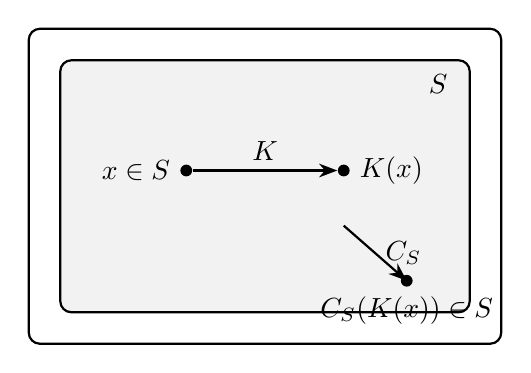
\begin{tikzpicture}[>=Stealth, node distance=1.4cm]
  \draw[rounded corners,thick] (-3,-2) rectangle (3,2);
  \draw[rounded corners,thick,fill=gray!10] (-2.6,-1.6) rectangle (2.6,1.6);
  \node at (2.2,1.3) {$S$};
  \node[circle,fill,inner sep=1.5pt,label=left:{$x\in S$}] (x) at (-1,0.2) {};
  \node[circle,fill,inner sep=1.5pt,label=right:{$K(x)$}] (kx) at (1,0.2) {};
  \draw[->,thick] (x) -- (kx) node[midway,above] {$K$};
  \draw[->,thick] (1,-0.5) -- (1.8,-1.2) node[midway,right] {$\clamp_S$};
  \node[circle,fill,inner sep=1.5pt,label=below:{$\clamp_S(K(x))\in S$}] (cs) at (1.8,-1.2) {};
\end{tikzpicture}
\caption{Forward closure and clamping.}
\end{figure}

\end{document}

\end{document}
